\documentclass{article}
\linespread{1.3}
\usepackage[margin=50pt]{geometry}
\usepackage{amsmath, amsthm, amssymb, amsthm, tikz, fancyhdr, float, graphicx, spverbatim, systeme}
\pagestyle{fancy}
\renewcommand{\headrulewidth}{0pt}
\newcommand{\changefont}{\fontsize{15}{15}\selectfont}

\fancypagestyle{firstpageheader}{
  \fancyhead[R]{
    \changefont
    \parbox[t]{4cm}{ % Adjust width as needed
      Michael Huang\\
      EN.625.633.81\\
      Homework 9
    }
  }
}

\begin{document}

\thispagestyle{firstpageheader}
{\Large 

\section*{1.}

\begin{figure}[H]
    \centering
    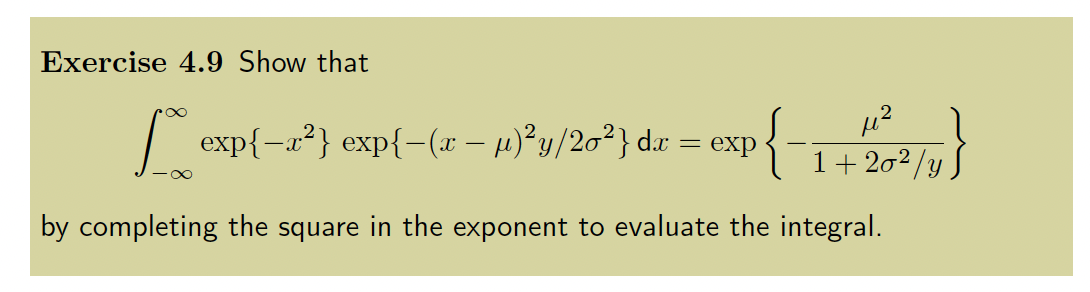
\includegraphics[width=0.75\textwidth]{Exercise4.9.png}
\end{figure}


}
{\Large 

\section*{2.}

\begin{figure}[H]
    \centering
    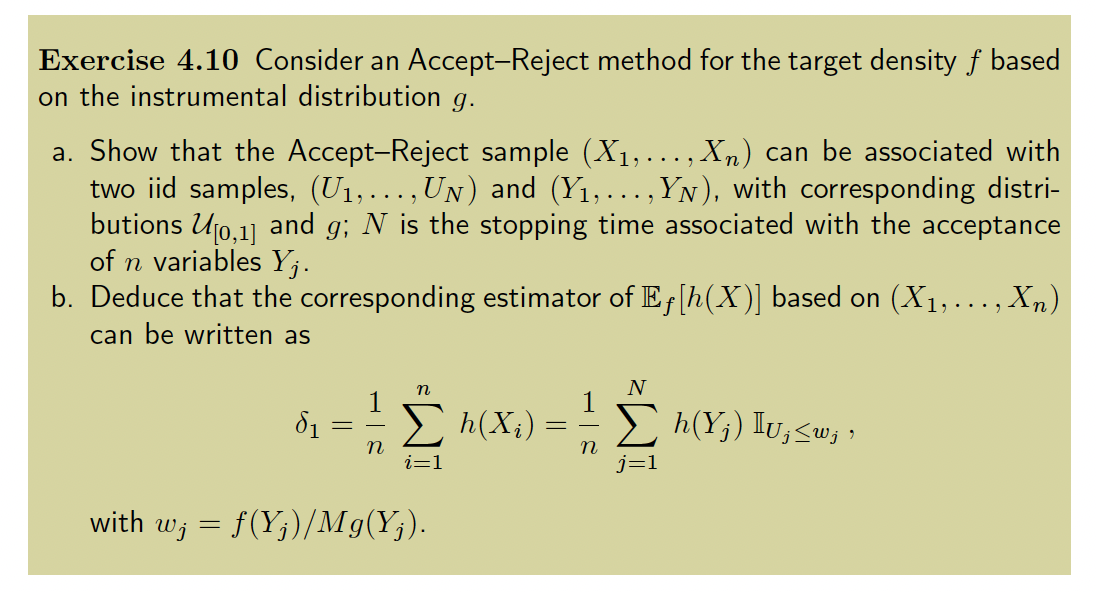
\includegraphics[width=0.75\textwidth]{Exercise4.10.png}
\end{figure}

\subsection*{(a)} 



\subsection*{(b)}



}
{\Large 

\section*{3.}

\begin{figure}[H]
    \centering
    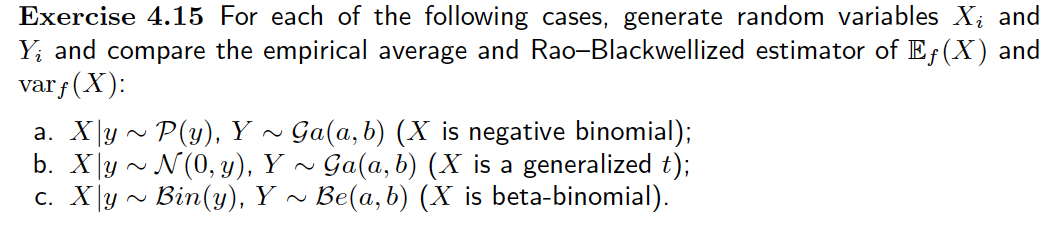
\includegraphics[width=0.75\textwidth]{Exercise4.15.png}
\end{figure}

\subsection*{(b)} 



\subsection*{(c)}



}
{\Large 

\section*{4.}

\begin{figure}[H]
    \centering
    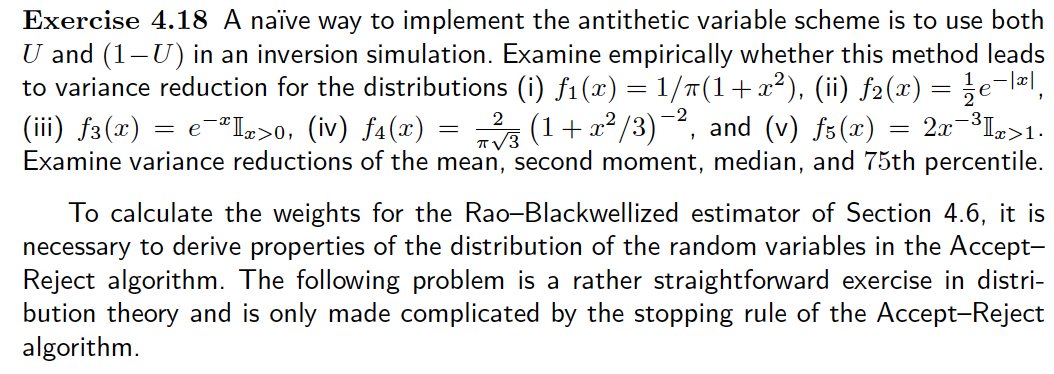
\includegraphics[width=0.75\textwidth]{Exercise4.18.png}
\end{figure}

\subsection*{(i)} 



\subsection*{(ii)}



\subsection*{(iv)}



}
{\Large 

\section*{5.}

Assuming that we use antithetic variables to estimate some parameter of the standard normal distribution, we must prove that the covariance between \(X_i\) and \(Y_i\) is -1.

}

\end{document}